\documentclass{lug}

\title{The Pythonic Way}
\author{Jack Rosenthal}
\institute{Mines Linux Users Group}

\usepackage{etoolbox}

\makeatletter
\patchcmd{\beamer@sectionintoc}{\vskip1.5em}{\vskip0.5em}{}{}
\makeatother

\begin{document}

\begin{frame}{Table of contents}
    \setbeamertemplate{section in toc}[sections numbered]
    \tableofcontents[hideallsubsections]
\end{frame}

\section{Background}

\begin{frame}{A Bit of History}
    \begin{itemize}[<+->]
        \item Python first appeared in early 1991. \emph{This means that Python
            is older than Java and Ruby.}
        \item Guido van Rossum (GvR, the creator of Python) designed his
            language with \textbf{emphasis on readability}.
        \item Python was named after \emph{Monty Python's Flying Circus}.
        \item The language quickly gained popularity because of its appeal to
            long-time UNIX/C hackers\footnote{See the Jargon File on hackers
            vs.  crackers}.
    \end{itemize}
\end{frame}

\begin{frame}{Python: The Perfect Companion to Linux}
    \begin{columns}
        \begin{column}{0.6\textwidth}
            \begin{itemize}[<+->]
                \item Easy to use without a domain specific IDE or editor
                \item On-line documentation with \texttt{pydoc} similar to
                    \texttt{man}
                \item UNIX system calls share the same name as in \texttt{libc}
                \item Fast and lightweight
                \item Very general purpose
                \item Easy to learn, but plenty to master
            \end{itemize}
        \end{column}
        \begin{column}{0.4\textwidth}
            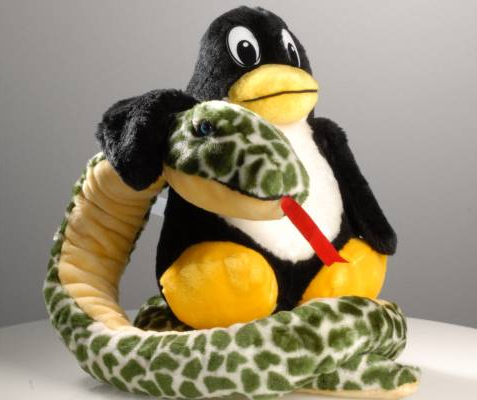
\includegraphics[width=\textwidth]{graphics/tux_on_python}
        \end{column}
    \end{columns}
\end{frame}

\begin{frame}{A Note on Python 2 and Python 3}
    Python 3 fixed many odds and ends from older versions of Python. When it
    was originally released, its usage was low due to many backwards
    incompatibilities. Now days, most modern projects use Python 3, so this
    issue is largely irrelevant.

    For the purposes of this presentation, we will be talking \emph{strictly of
    Python 3}.

    \pause
    \medskip

%    \begin{block}{Setting The Default}
%        \small
%        Debian/Ubuntu systems have Python 2 as the default, to switch this to
%        Python 3, run this command:
%
%        \texttt{\# update-alternatives --install /usr/bin/python \textbackslash \\
%        \phantom{\#} python /usr/bin/python3 2}
%    \end{block}

    \begin{block}{Setting The Default}
        \small
        Some systems have Python 2 as the default, the general solution is to
        alias \texttt{python} to \texttt{python3}. Add this to your shell's
        \emph{rc file}.

        \texttt{alias python=python3}
    \end{block}
\end{frame}

\begin{frame}{A Simple Example}
    The classical \emph{Fizz Buzz} problem: for all the numbers from 1 to 100,
    print \texttt{Fizz} if the number is divisible by 3, \texttt{Buzz} if
    divisible by 5, \texttt{Fizz Buzz} if divisible by 3 and 5, and the number
    otherwise.

    \inputminted{python3}{examples/fizzbuzz.py}
\end{frame}

\begin{frame}{The Zen of Python}
    PEP-20 lists a series of principles for which the language was designed
    under. Typing \texttt{import this} at the Python interpreter will show you
    the zen:

    \inputminted{pycon}{console/importthis.py}

    \pause

    In short, Python was designed with careful thought about how to make it
    \emph{Pythonic}.
\end{frame}

\section{Python Style}

\begin{frame}{A Foolish Consistency is the Hobgoblin of Little Minds}
    \begin{itemize}[<+->]
        \item GvR makes a point: \emph{code is read more often than it is
            written}, so \textbf{readability counts}.
        \item Python is one of the few languages with a style guide (PEP-8)
            since there is a huge amount of Python code out there and the
            language's core principle is readability.
        \item Thus, it's important to follow Python's official style whenever
            possible
    \end{itemize}
    \pause[\thebeamerpauses]
    \begin{block}{Legacy Code}
        \small
        It should be noted that when working on a project that was started
        before the ages of PEP-8, generally they have their own style guide and
        you should follow that instead.  Otherwise, it would be generally
        considered unacceptable to not follow PEP-8.
    \end{block}
\end{frame}

\begin{frame}{Naming}
    \begin{itemize}[<+->]
        \item Python uses \texttt{snake\_case} for variable names, function
            names, method names, and module names
        \item You should avoid using underscores when possible to improve
            readability (eg.\ \texttt{randint} is better than
            \texttt{rand\_int}, as the naming is obvious without the
            underscore).
        \item When there are conflicts with builtin keywords and a better name
            is not possible, an underscore should be appended to the variable
            name (eg.\ \texttt{class\_})
        \item Class names should be typed in \texttt{CapWords}
        \item Function, method, and class names should describe the
            interface rather than the implementation.
        \item Private methods and variables should start with an underscore.
    \end{itemize}
\end{frame}

\begin{frame}{Indentation}
    As Python uses the indentation of the text to denote scope, consistency of
    indentation is critically important. PEP-8 recommends the following:
    \begin{itemize}[<+->]
        \item Use 4 spaces per indentation level, \textbf{never use hard tabs}.
        \item On multiline function calls, list literals, etc., the arguments
            should be aligned and indented from the rest of the text. ``Hanging
            indent'' is acceptable as well.
        \item Multiline \texttt{if}/\texttt{while} etc.\ should be indented to
            align with the top line
    \end{itemize}
\end{frame}

\begin{frame}[fragile]{Other Pet Peeves}
    \begin{itemize}[<+->]
        \setlength\itemsep{5mm}
        \item Keep lines to 79 characters\footnote{It's OK to go to 90 or 100
            if everyone in your project agrees.}
        \item Avoid extraneous whitespace inside parentheses, brackets, and
            braces

            \medskip

            \begin{minipage}{\linewidth}
            \begin{minted}{python3}
                Yes: spam(ham[1], {eggs: 2})
                No:  spam( ham[ 1 ], { eggs: 2 } )
            \end{minted}
            \end{minipage}

        \item Don't use parentheses on \texttt{if}/\texttt{while} etc.\ like
            you might in C-like languages

            \medskip

            \begin{minipage}{\linewidth}
            \begin{minted}{python3}
                Yes: if i < 3:
                No:  if(i < 3):
            \end{minted}
            \end{minipage}

    \end{itemize}
\end{frame}

\begin{frame}[fragile]{Truthiness}
    Anything \texttt{None}, \texttt{False}, zero, or an empty sequence/mapping
    will implicity be false, and you \emph{should} take advantage of that.

    \begin{minted}{python3}
        Disgusting: if mybool == False:
        Pythonic:   if mybool:
    \end{minted}

    \begin{minted}{python3}
        Disgusting: if mydata == None:
        Pythonic:   if mydata:
    \end{minted}

    \begin{minted}{python3}
        Ehh:        if mynumber != 0:
        Pythonic:   if mynumber:
    \end{minted}

    \begin{minted}{python3}
        Ugly:       if len(mylist) == 0:
        Better:     if not len(mylist):
        Pythonic:   if not mylist:
    \end{minted}
\end{frame}

\begin{frame}{Comments}

    \textit{%
        Every comment in the source code is a personal failure of the
        programmer, because it proves that he didn’t manage to express the
        purpose of the code fragment with the programming language itself.
    }
    \hspace*\fill{\small--- Uncle Bob}

    \begin{center}
        
\includegraphics[width=0.7\linewidth]{graphics/unclebob}
    \end{center}

    \small
    \textbf{Take Home:} Comments are important when they are needed, but you
    should try and make your code readable instead.

\end{frame}

\begin{frame}{Concluding Remarks on Coding Style}
    \begin{center}
        \bfseries
        \Huge
        Readability Counts!
    \end{center}

    \begin{center}
        No really, it is of utmost importance that Python code be readable
        \textbf{by following the guidelines of PEP-8}. You should read through
        PEP-8 before getting serious with Python.
    \end{center}
\end{frame}

\section{Language Structures}

\begin{frame}{Literals}
    \inputminted{python3}{examples/literals.py}
\end{frame}

\begin{frame}{Selection}
    Python's primary structure for selection is \texttt{if}:

    \inputminted{python3}{examples/ifexample.py}

    \pause

    There's also a ternary operator (good for simple conditionals):

    \inputminted{python3}{examples/ternary.py}

\end{frame}

\begin{frame}{Why no \texttt{switch}/\texttt{case}?}

    \begin{onlyenv}<1>
        Most \texttt{switch}/\texttt{case} statements over-complicate what could be
        done in a single line using a dictionary. Where this is not the case, you
        really shouldn't be using a \texttt{switch} anyway.
    \end{onlyenv}

    \begin{onlyenv}<2>
        \textbf{\large An Example \texttt{switch} in C}\par
        \inputminted{c}{examples/switch.c}
    \end{onlyenv}

    \begin{onlyenv}<3>
        \textbf{\large The Pythonic Way}\par
        \inputminted{python3}{examples/dictswitch.py}
    \end{onlyenv}

\end{frame}

\begin{frame}{Iteration}
    Python provides your traditional \texttt{while} loop, the syntax is similar
    to \texttt{if}:

    \inputminted{python3}{examples/while.py}

    \pause

    But under most cases, the \textbf{range-based} \texttt{for} loop is preferred:

    \inputminted{python3}{examples/for.py}

    {\small%
    It should be noted that Python's \texttt{for} loop is strictly range-based,
    unlike C's \texttt{for} loop which is really just a fancy \texttt{while}
    loop.
    }
\end{frame}

\begin{frame}{\texttt{while}-\texttt{else} and \texttt{for}-\texttt{else}}
    Little known is the ability to pair an \texttt{else} block with
    \texttt{for} and \texttt{while}. The block will be executed \emph{only if}
    the loop finishes \textbf{without \texttt{break}ing}.

    An example of this can be seen below:
    \inputminted{python3}{examples/forelse.py}
\end{frame}

\begin{frame}{Slicing}
    \inputminted{python3}{examples/slicing.py}
\end{frame}

\begin{frame}[fragile]{Tuple Expansion \& Collection}
    Multiple assignments work like so:
    \begin{minted}{python3}
        names = ("R. Stallman", "L. Torvalds", "B. Joy")
        a, b, c = names
    \end{minted}

    \pause

    \texttt{*} can be used to collect a tuple:
    \begin{minted}{python3}
        # drop the lowest and highest grade
        grades = (79, 81, 93, 95, 99)
        lowest, *grades, highest = grades
    \end{minted}

    \pause
    The same can be done to expand a tuple in a function call:
    \begin{minted}{python3}
        print(*grades)
    \end{minted}

\end{frame}

\begin{frame}{Functions}
    Functions are \emph{first-class citizens} in Python:
    \inputminted{pycon}{console/function.py}

    \pause

    Functions can also be written anonymously as \texttt{lambda}s:
    \inputminted{pycon}{console/lambda.py}

    \pause
    \small
    In this case, the first style is preferred. It's a bit easier to read, not
    to mention it's actually named.

\end{frame}

\begin{frame}{\texttt{*args}, \texttt{**kwargs}}
    Python allows you to define functions that take a variable number of
    positional (\texttt{*args}) or keyword (\texttt{**kwargs}) arguments. In
    principle, this really just works like tuple expansion/collection.

    \pause

    \inputminted{python3}{examples/args_kwargs.py}
\end{frame}

\begin{frame}{Generator Functions}
    \small
    Python provides a special kind of function which \texttt{yield}s rather
    than \texttt{return}s. This \textbf{generator function} is effectively an
    efficient iterable.

    Consider the \texttt{range} function we have been using\footnote{This is
    actually a simplification}:
    \inputminted{python3}{examples/rangefunction.py}

    \pause

    As we will see later on, generator functions are a certain kind of the more
    generic \textbf{generator}.

\end{frame}

\section{Object Oriented Programming}

\begin{frame}{Classes}
    A simple class can be defined like so:
    \inputminted{python3}{examples/simpleclass.py}

    \pause

    A few things to notice:
    \begin{itemize}
        \item \texttt{\_\_init\_\_} is the initializes the object. It's
            actually what is called a \textbf{magic method}
        \item All the methods of the class take a parameter \texttt{self}, the
            object you are working on
    \end{itemize}
\end{frame}

\begin{frame}{Magic Methods}

    \textbf{Magic methods} are methods with certain names that allow you to
    bind features of your class to certain Python features.

    \begin{itemize}[<+->]
        \item \texttt{\_\_init\_\_} was the simple example we just saw.
        \item \texttt{\_\_del\_\_} gets called when your object gets
            destructed.
        \item \texttt{\_\_lt\_\_}, \texttt{\_\_eq\_\_}, etc.\ allow you to
            define comparisons.
        \item \texttt{\_\_len\_\_} binds into Python's \texttt{len($\cdot$)}
        \item There's far more than I can mention here. Read the docs!
    \end{itemize}

    \pause[\thebeamerpauses]

    \begin{block}{Why do this rather than \texttt{.equals()},
        \texttt{.length()} and such?}
        \small
        \emph{%
        In the face of ambiguity, refuse the temptation to guess.
        There should be one -- and preferably only one -- obvious way to do it.
        }

        Avoid \texttt{.length()}, \texttt{.getLength()}, \texttt{.size()}
        inconsistencies
    \end{block}

\end{frame}

\begin{frame}{Properties}
    \textbf{Readability counts}, so Python provides a way to avoid writing
    ``getters and setters'' when unnecessary.

    \pause

    In Java, it's nearly impossible to make everything public, since changing
    a class to use getters and setters would require a change of everything
    that interfaces with it.

    \pause

    Python's properties allow you to make your variable public to begin with,
    and then write getters and setters only once they are needed to actually
    check something.

\end{frame}

\begin{frame}{Using Properties}

    \scriptsize

    \begin{columns}
        \begin{column}{0.6\textwidth}
            \begin{onlyenv}<1>
                \inputminted{python3}{examples/camerasensorsimple.py}
            \end{onlyenv}
            \begin{onlyenv}<2>
                \inputminted{python3}{examples/camerasensorproperty.py}
            \end{onlyenv}
        \end{column}
        \begin{column}{0.4\textwidth}
            \inputminted{python3}{examples/camerasensorusage.py}
        \end{column}
    \end{columns}

\end{frame}

\section{Decorators}

\begin{frame}{Decorators}
    \texttt{@property} as we just saw is what is called a decorator. Decorators
    are really just a pretty way to wrap functions using functions that return
    functions.

    \pause

    Both the following are equivalent:
    \inputminted{python3}{examples/decorator_equiv.py}
\end{frame}

\begin{frame}{Defining Decorators}
    When defining wrapper functions, you should decorate it with \texttt{wraps}
    from \texttt{functools}, this will keep attributes about the function.
    \inputminted{python3}{examples/decorator_logging.py}
\end{frame}

\begin{frame}{Decorators in the Wild: Dynamic Programming}
    \texttt{lru\_cache} from \texttt{functools} can be a quick way to make a
    recursive function with a recurrence relation fast. Here's an example:
    \pause
    \inputminted{python3}{examples/fibonacci.py}
\end{frame}

\begin{frame}{Decorators in the Wild: Welford's Equations}
    Welford's Equations are a one-pass mean and standard deviation algorithm.
    One important property is that we won't have to store the results in a
    list.

    \pause

    Our goal will be to implement a decorator we can use like this:
    \inputminted{python3}{examples/welford_usage.py}
\end{frame}

\begin{frame}{Decorators in the Wild: Implementing Welford}
    \small
    The key here is that we can make callable objects using
    \texttt{\_\_call\_\_}.

    \tiny
    \inputminted{python3}{examples/welford_class.py}

\end{frame}

\begin{frame}{More Decorator Tricks}
    \begin{itemize}[<+->]
        \item Decorators can wrap classes as well as functions. A practical
            example might be creating a decorator which adds attributes of a
            class to a database (a \texttt{@model} decorator?)
        \item When multiple decorators are typed, they are applied bottom-up.
    \end{itemize}
\end{frame}

\section{Generators \& Comprehensions}

\begin{frame}[fragile]{Generator Expressions}
    Remember the generator function from earlier? Generators can be written
    inline, these are called \textbf{generator expressions}.

    \medskip

    \begin{minipage}{\linewidth}
        \centering
        \RecustomVerbatimEnvironment{Verbatim}{BVerbatim}{}
        \inputminted{python3}{examples/generator_basic.py}
    \end{minipage}

    \medskip

    \pause

    There's two parts to a generator expression:
    \begin{enumerate}[<+->]
        \item Performing something for every element with \texttt{for...in}.
        \item Selecting a subset of elements to operate on with \texttt{if}.
            This part is optional.
    \end{enumerate}

    \pause[\thebeamerpauses]

    \medskip

    \begin{block}{The Pythonic Way}
        \small \itshape
        Generator expressions are key to the art of Python. Without extensive
        knowledge of generator expressions, one will forever be a novice
        Pythonist.
    \end{block}

\end{frame}

\begin{frame}{Expression Syntax}
    \inputminted{python3}{examples/generator_syntax.py}
    Notice the loops are evaluated outside-in.
\end{frame}

\begin{frame}[fragile]{Applications of Generator Expressions}
    \begin{itemize}[<+->]
        \setlength\itemsep{10pt}
        \item Summing ASCII values of a string

            \begin{minipage}{\linewidth}
                \small
                \begin{minted}{python3}
                    sum(ord(c) for c in s)
                \end{minted}
            \end{minipage}

            {\small Note that the double-parentheses can be omitted.}

        \item File readers
            \smallskip

            \begin{minipage}{\linewidth}
                \small
                \begin{minted}{python3}
                    reader = (float(line) for line in f)
                    while processing_queue:
                        process(next(reader))
                \end{minted}
            \end{minipage}

        \item Hash Function pRNGs
            \smallskip

            \begin{minipage}{\linewidth}
                \small
                \begin{minted}{python3}
                    rng = (hashfunc(x)/MAXHASH for x in count())
                    diceroll(next(rng))
                \end{minted}
            \end{minipage}

        \item The possibilities are endless!
    \end{itemize}
\end{frame}

\begin{frame}{List Comprehensions}
    Building lists in a syntax like generator expressions can be done simply by
    using square brackets.
    \medskip

    \inputminted{python3}{examples/generator_basic_lc.py}

    \pause

    \medskip

    \begin{block}{Non-comprehensive Alternative}
        This is an alternative to the \textbf{bad programming} edition:

        \smallskip

        \begin{minipage}{\linewidth}
        \inputminted{python3}{examples/generator_basic_lc_disgusting.py}
        \end{minipage}

        \smallskip

        {\small Please avoid writing \textbf{absolute garbage} like this
        to initialize a data structure! It's convoluted and slow!}
    \end{block}

\end{frame}

\begin{frame}{Generic Comprehensions}
    The same comprehension syntax can be applied to other data structures like
    so:
    \inputminted{python3}{examples/generic_comprehensions.py}
\end{frame}

\section{Functional Programming}

\begin{frame}{Functional Programming}
    \begin{columns}
        \begin{column}{0.7\linewidth}
            \begin{itemize}[<+->]
                \item High-order functions
                \item We can do a lot in very few lines
                \item Allow us to mathematically prove our algorithms correct, that's
                    better than any finite amount of unit tests!
                \item Decorators are a little piece of functional programming
                \item Generator expressions are also a form of functional
                    programming
            \end{itemize}
        \end{column}
        \begin{column}{0.3\linewidth}
            \hspace*{25pt}
\includegraphics[width=\textwidth]{graphics/hammer.png}
        \end{column}
    \end{columns}
\end{frame}

\begin{frame}{\texttt{min}/\texttt{max}}
    \texttt{min}/\texttt{max} gets the minimum or maximum value from an
    iterable, optionally using a key function to select by.

    \pause

    \textbf{Example:}
    \begin{minipage}{\linewidth}
        \centering
        \RecustomVerbatimEnvironment{Verbatim}{BVerbatim}{}
        \inputminted{python3}{examples/minmax.py}
    \end{minipage}

    \medskip
    \pause

    \begin{block}{The \emph{Bad Programming} Version}
        \begin{minipage}{\linewidth}
            \inputminted{python3}{examples/minmax_bad.py}
        \end{minipage}

        {\centering\emph{Don't do this crap!}\par}
    \end{block}
\end{frame}

\begin{frame}{\texttt{zip}}
    \texttt{zip} creates a \textbf{iterator} over the $n$th element of each of
    it's arguments (which are iterables).

    \pause

    \textbf{Example:}
    \inputminted{python3}{examples/zip.py}

    \pause

    \begin{block}{\emph{Pro Tip:} Iterating over the columns of a 2D matrix}
        \begin{minipage}{\linewidth}
            \inputminted{python3}{examples/zip_matrix.py}
        \end{minipage}
    \end{block}
\end{frame}

\begin{frame}{Other Functional Things}
    \begin{itemize}[<+->]
        \item \texttt{map(func, *iterables)}, which calls \texttt{func(*t)} for
            all \texttt{t} in \texttt{zip(*iterables)}. Note that \texttt{map}
            is completely unnecessary as the same can be done using generator
            expressions. Under a few cases, it may be better to use
            \texttt{map} to improve readability.
        \item \texttt{reduce(func, sequence)} which reduces a sequence by
            calling \texttt{func(func(func(a, b), c), ...)}. This is useful for
            taking the product of a sequence (use \texttt{operator.mul})
    \end{itemize}
\end{frame}

\begin{frame}{Recommended Reading}
    The \textbf{Functional Programming HOWTO} page in the Python documentation
    has some very useful tips for functional programming.

    \url{https://docs.python.org/howto/functional.html}
\end{frame}

\section{Useful Libraries}

\begin{frame}{\texttt{itertools}}
    \begin{columns}
        \begin{column}{0.7\linewidth}
            \begin{itemize}[<+->]
                \item Built into Python's standard library
                \item Features common generator functions
                \item Features generator functions for iterating over various
                    combinatorics, eg.\ permutations
            \end{itemize}
        \end{column}
        \begin{column}{0.3\linewidth}
            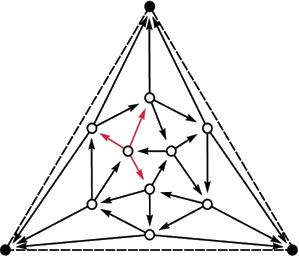
\includegraphics[width=\linewidth]{graphics/graph}
        \end{column}
    \end{columns}

    \pause[\thebeamerpauses]
    \bigskip

    \begin{block}{\emph{Example:} Exhaustive Search Over Permutations}
        \begin{minipage}{\linewidth}
            \tiny
            \inputminted{python3}{examples/exhaustive.py}
        \end{minipage}
    \end{block}
\end{frame}

\begin{frame}{Requests}
    \begin{columns}
        \begin{column}{0.7\linewidth}
            \begin{itemize}[<+->]
                \item Useful library to do make HTTP requests easy
                \item Requests is the only \emph{Non-GMO} HTTP library for
                    Python, safe for human consumption.
            \end{itemize}
        \end{column}
        \begin{column}{0.3\linewidth}
            
\includegraphics[width=\linewidth]{graphics/requests}
        \end{column}
    \end{columns}

    \pause[\thebeamerpauses]
    \bigskip

    \begin{block}{Behold! The power of Requests!}
        \begin{minipage}{\linewidth}
            \tiny
            \inputminted{pycon}{console/requests_ex.py}
        \end{minipage}
    \end{block}
\end{frame}

\begin{frame}{Bottle: Really Simple Web Framework}
    \begin{columns}
        \begin{column}{0.7\linewidth}
            \begin{itemize}[<+->]
                \item Provides routing and convenient access to data
                \item Built in HTTP server, or use any WSGI-compatible web
                    server
                \item Very lightweight, only a couple thousand lines of code
            \end{itemize}
        \end{column}
        \begin{column}{0.3\linewidth}
            
\includegraphics[width=\linewidth]{graphics/bottle}
        \end{column}
    \end{columns}

    \pause[\thebeamerpauses]
    \bigskip

    \begin{block}{A \emph{Hello, World!} App}
        \begin{minipage}{\linewidth}
            \tiny
            \inputminted{python3}{examples/bottle_ex.py}
        \end{minipage}
    \end{block}
\end{frame}

\begin{frame}[standout]
    \Huge
    Library Suggestions?
\end{frame}

\section{Learning Resources}

\begin{frame}{Learning Resources}
    \begin{itemize}[<+->]
        \item The Python documentation is excellent, and includes many
            tutorials and howtos that may be more readable to a beginner
        \item My slides\footnote{These slides aren't complete without someone
            to teach them.} from this past summer are online at
            \url{https://coding.campinc.com}, these might be better for someone
            with zero programming experince
        \item Online courses? I haven't tried any.
        \item \textbf{The Python Cookbook} by \emph{David Beazely} and
            \emph{Brian K. Jones} is a good book for seasoned Pythonists
    \end{itemize}
\end{frame}

\begin{frame}[standout]
    \Huge
    Questions?
\end{frame}

\end{document}
